\chapter{Introduction}\label{Chap1}
\echapter{Introduction}
In the microelectronics industry, the chip technology is rapidly evolving towards miniaturization in accordance to the Moore's law. Owing to this miniaturization trend in the chip technology, the reliability of solder joints used in the electronic packaging has been considered as a significant topic.  Among the several aspects of reliability, the microbubbles and intermetallic compounds(IMCs), which get formed and grow considerably during the reflow soldering need special attention. With the dimensions of these bubbles being several values lower than millimeters length scale, the experimental study need to assisted by computational methods for a better understanding of the physical properties and phenomena.

\section{Background}\label{Chap1_01}
\esection{Background}

\subsection{Planar Microbubbles} \label{Chap1_01_01}
\esubsection{Planar Microbubbles}
Solder voiding has been a common phenomenon in mass reflow soldering processes used in the electronic packaging technologies, being variously characterized as process anomalies, process indicators and/or solder defects. A solder void can be defined as a hole or enclosed volume of space within the solder joint that lacks solder material ~\cite{TLLewis:2012}. The planar microbubbles or microvoids, having size smaller than 1-2 millimeters in diameter and being located in one plane at the substrate-to-solder interface above the intermetallic compound, are considered to be the risk for reliability failures of BGA and other solder joints ~\cite{RAspandiar:2006}. Most of the cases of planar microbubbles are associated with the gaseous materials resulting from the flux during reflow soldering.

\subsection{Intermetallic Compounds} \label{Chap1_01_02}
\esubsection{Intermetallic Compounds}
The compounds that are formed at the interface of the Sn rich solder and Cu substrate  are called the intermetallic compounds (IMCs). Cu$_6$Sn$_5$ and Cu$_3$Sn are the commonly known IMCs in the Sn and Sn-0.7Cu solder system.  Owing to the brittle nature of these compounds,the thickness of the IMC is considered an important reliability parameter ~\cite{MLHuang2015}. For most of the design purpose, solder systems are supposed to have a relatively thinner IMC.



\section{Motivation}\label{Chap1_01}
\esection{Motivation}
As most of the electronic devices are undergoing the trend of miniaturization, study of the reliability issues in electronic packaging assemblies and solder joints has acquired a notable significance among the researchers.As the solder microvoids, decrease the contact area of the solder interface and weaken the solder joints, they are the one of the key issues regarding the reliability of solder joints. The simulation of the growth behavior of solder bubbles and voids through computational methods can be a good approach when the experimental study about the solder voiding is at the crossroads. In relation to the IMCs of solder joints in real practice, the phenomena of thermomigration and electromigration interfere the growth pattern of the compounds. Thus, the assessment of the dimensional changes of the IMCs under the externally applied temperature  and electric field  gradients can contribute to the knowledge of design parameters in soldering procedures. In this connection, the implementation of numerical models can assist in better  as well as meticulous understanding of the physical phenomena and material properties.

\section{Summary of Contributions}\label{Chap1_02}
\esection{Summary of Contributions}

The contributions of this dissertation, which are elaborated throughout this dissertation, are listed as follows:
\begin{enumerate}
    \item \textbf{ASNETs middleware framework}
    \\
    Middleware framework for wireless networks have been a topic of research for several years. However, there is no formal data management system framework to date that consolidates all current research in this area. This is considered a potential weakness of the research field. For example, the design of proposed data management protocols remains difficult, mainly due to the lack of system framework upon which the design could be based. Such system framework will provide the background for design and evaluation of middleware protocols. It will also help to provide metrics for assessing the effectiveness of an ASNET middleware protocol as well as its performance.
        \begin{itemize}
            \item We provide theoretical model of online social behavior and dynamic network information to represent the relationship between users using a social graph.
            \item We present a method to understand the social metrics usage of the protocols.
            \item we propose an ASNETs framework which integrates layers from sensing level to application level.
        \end{itemize}
    \item \textbf{Community partition aware data replication scheme for ASNETs with the exploitation of social relationships}
    \\
    A new data replication protocol called ComPAS (community-partition aware replica allocation method) is proposed initially. This method can significantly improve ASNETs performance by exploiting social relationship while replicating in the community to achieve better efficiency and consistency while keeping the replica relocation cost as low as possible.
        \begin{itemize}
            \item We model the data management middleware system for ASNETs with underlying different modules.
            \item We outline social relationship considerations as a social behavior for the exploitation of group mobility model.
            \item We provide an overview and selection on existing replica allocation approaches, that ease the impact of ASNETs connectivity nature and improve data availability ratio.
            \item We derive the average read cost for the original data storage space in a community without replication and also calculate the optimum Read Cost Reduction (RCR).
            \item We devise a replica allocation algorithm based on the proposed model and derived formulas.
            \item We choose an optimum approach and provide a comparison based on metrics such as read cost, relocation period, number of mobility group and efficiency of consistency management.
        \end{itemize}
    \item \textbf{An optimal community-based event dissemination with load balancing mechanisms for ASNETs }
    \\
    A community-based load balancing protocol called Co-Lab is proposed, that seeks to improve the network performance by clustering brokers in a community taking interest similarity and filter replication into consideration. It attempts to effectively achieve a more consistent and uniform load distribution among brokers and to circumvent the occurrence of highly overloaded brokers.
        \begin{itemize}
            \item We introduce a community-based event dissemination and load balancing with a fault-tolerance mechanism considering community formation, event dissemination, broker clustering based on interest similarity, replication, and load distribution.
            \item We design a possible load balancing algorithm by exploiting interest similarity and integrating filter-based functionality within each multicast group that achieves fair load distribution among each broker as well as reducing the overall load distribution.
            \item We formulate and derive the community formation system of the network and calculating the number of brokers, publishers and subscribers that should be involved in each community.
            \item We present an event dissemination algorithm for Inter-Community and Intra-Community phases, while balancing the load among brokers.
            \item We design a broker clustering and filter replication mechanism in the community.
            \item We conduct evaluation to verify the performance of the proposed approach. For evaluation, we generated an appropriate social graph model which substantiates the advantages of the socially-aware design of our system.
\end{itemize}
    \item \textbf{Bacteria social behavior inspired algorithm to detect and mitigate the impact of selfish users in ASNETs}
    \\
    A biologically inspired algorithm to detect and mitigate the impact of selfish users on performance and efficiency of ASNETs. Its design considers social willingness (that depends on depth of social relationship among users) as a social behavior and bacteria chemical products as a counter to achieve optimal ASNETs performance. Counter is a parameter attached to individual user counting successful data operations performed in relation with others. Using social willingness and counter, BoDMaS assesses and classifies users, and counteracts their selfishness.
        \begin{itemize}
            \item We model how to map the bacteria mechanism into our solution and how our solution is motivated by behavior of bacteria in performing collaborative tasks.
            \item We consider social willingness and a biologically inspired mechanism (chemical products of bacteria) in ASNET data replication operations to detect and classify users as either cooperative or selfish.
            \item We present a BoDMaS system architecture, which is made up of behavior assessment, user classification, and user selection \& reaction components.
            \item We demonstrate that the functional interaction among BoDMaS components can effectively detect selfishness.
            \item We conduct simulations by applying important performance and efficiency metrics such as accessibility degree, detection rates, and network load balance to validate the BoDMaS effectiveness.
\end{itemize}
\end{enumerate}

\section{Organization of the Dissertation}\label{Chap1_03}
\esection{Organization of the Dissertation}
\begin{figure}[h]
\begin{center}
  \begin{tabular}{c}
  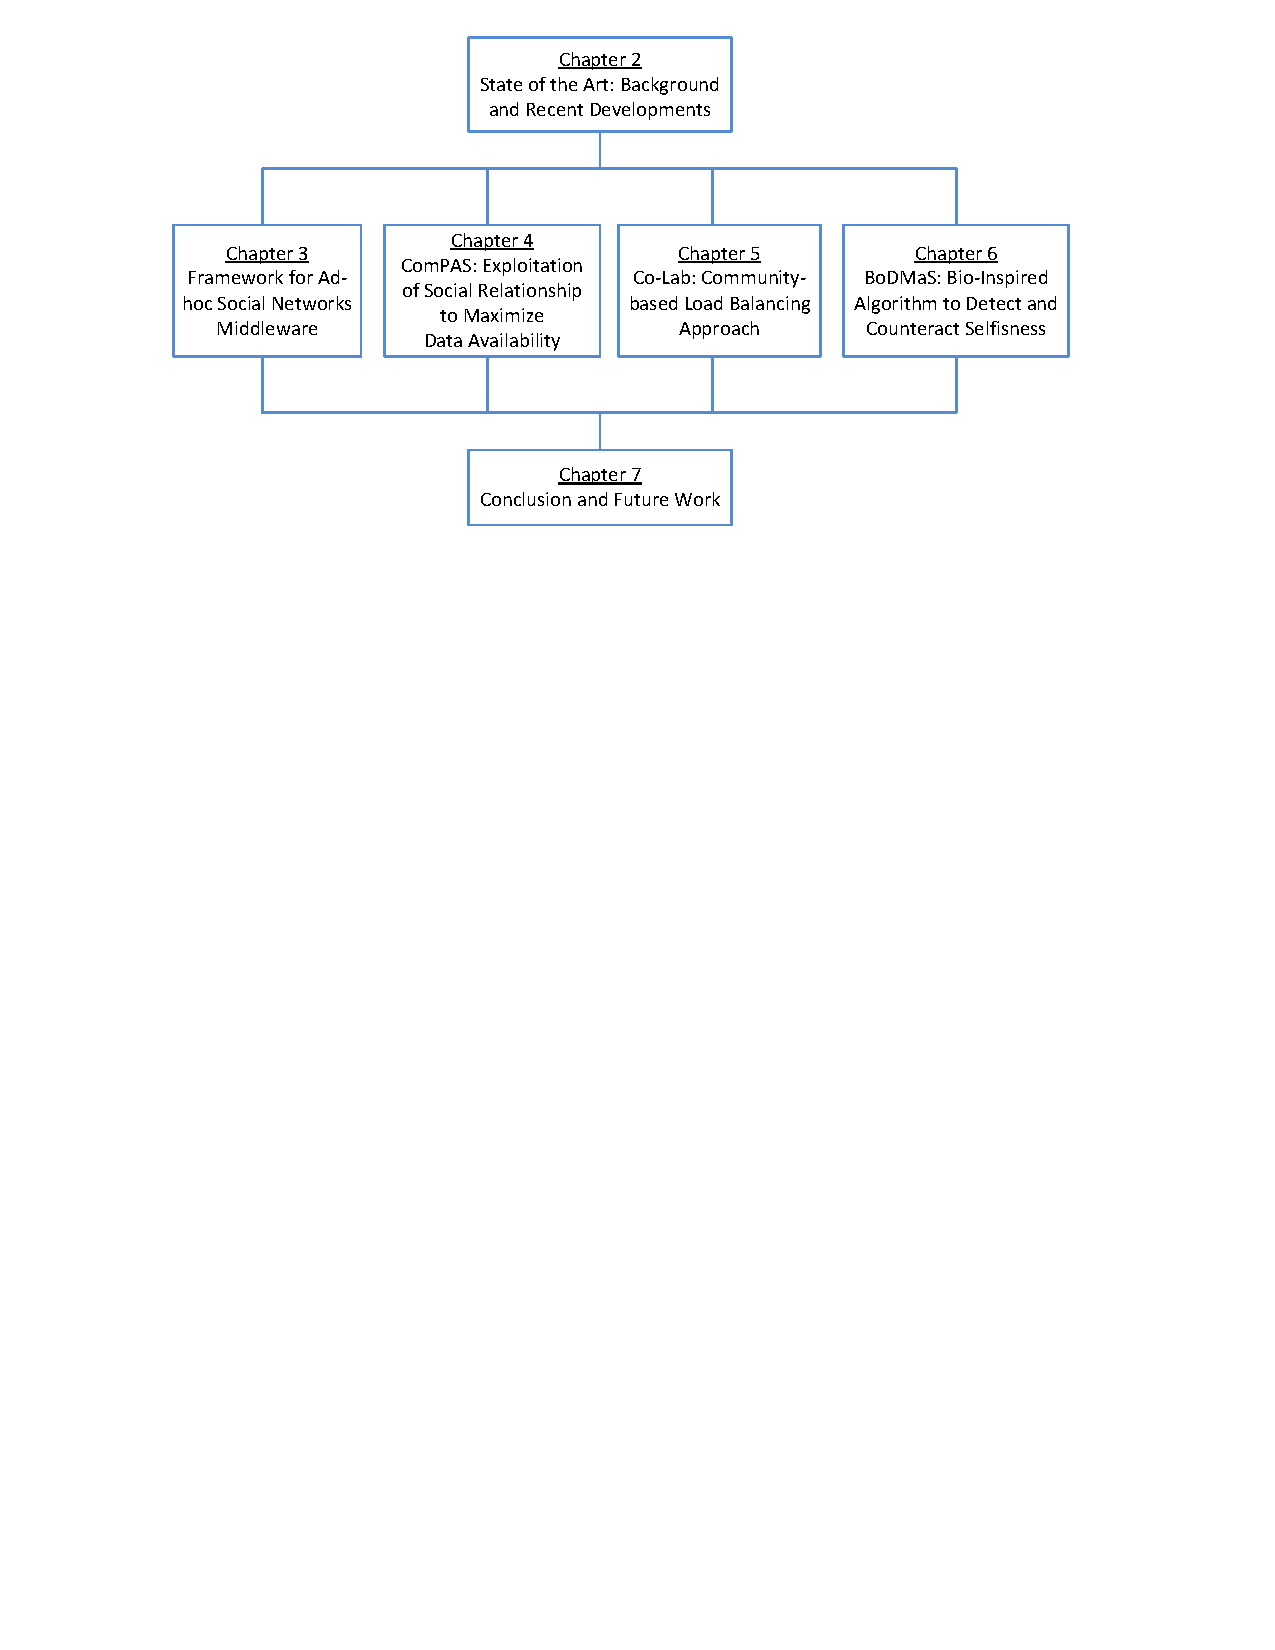
\includegraphics[width=0.856\textwidth]{Chap1-Fig2.pdf}
  \end{tabular}
  \caption{The organization of the remainder of the dissertation.}
\end{center}
\end{figure}
The remainder of the dissertation is organized as shown in Fig. 1.2: Chapter 2 lays a theoretical state of the art background for the following work, including introductions to user social behaviors, user mobility, middleware solutions for ad-hoc social networks, data replication, load balancing and user selfishness. Chapter 3 provides an ASNET middleware framework and overview of the relation of the layers as well as the protocols. Chapter 4 presents a social community partition aware replica allocation scheme that exploits users' relationship. In Chapter 5, we propose an optimal community-based load-balancing method. Chapter 6 provides bio-inspired algorithm to detect and counteract selfishness in ASNETs. Chapter 8 concludes the dissertation and discusses future research directions.

To provide an overall picture of the dissertation content, we created a dependency graph among chapters (Fig. 1.3) in which arrows suggest dependencies between chapters. Based on the dependency graph, therefore, a reader can start with Chapter 2 (state of the art: background and recent developments), and it is recommended that he or she read Chapters 3 (framework for ad-hoc social networks middleware) and 4 (ComPAS) before Chapter 5 (Co-Lab) and Chapter 6 (BoDMaS). We have also color-coded chapter boxes that are of the same level of importance and abstraction. The darkest chapters are the essentials of this dissertation, and the lightest boxes are those chapters that are more applied and have materials that are built on the foundation of other chapters.

\begin{figure}[h]
\begin{center}
  \begin{tabular}{c}
  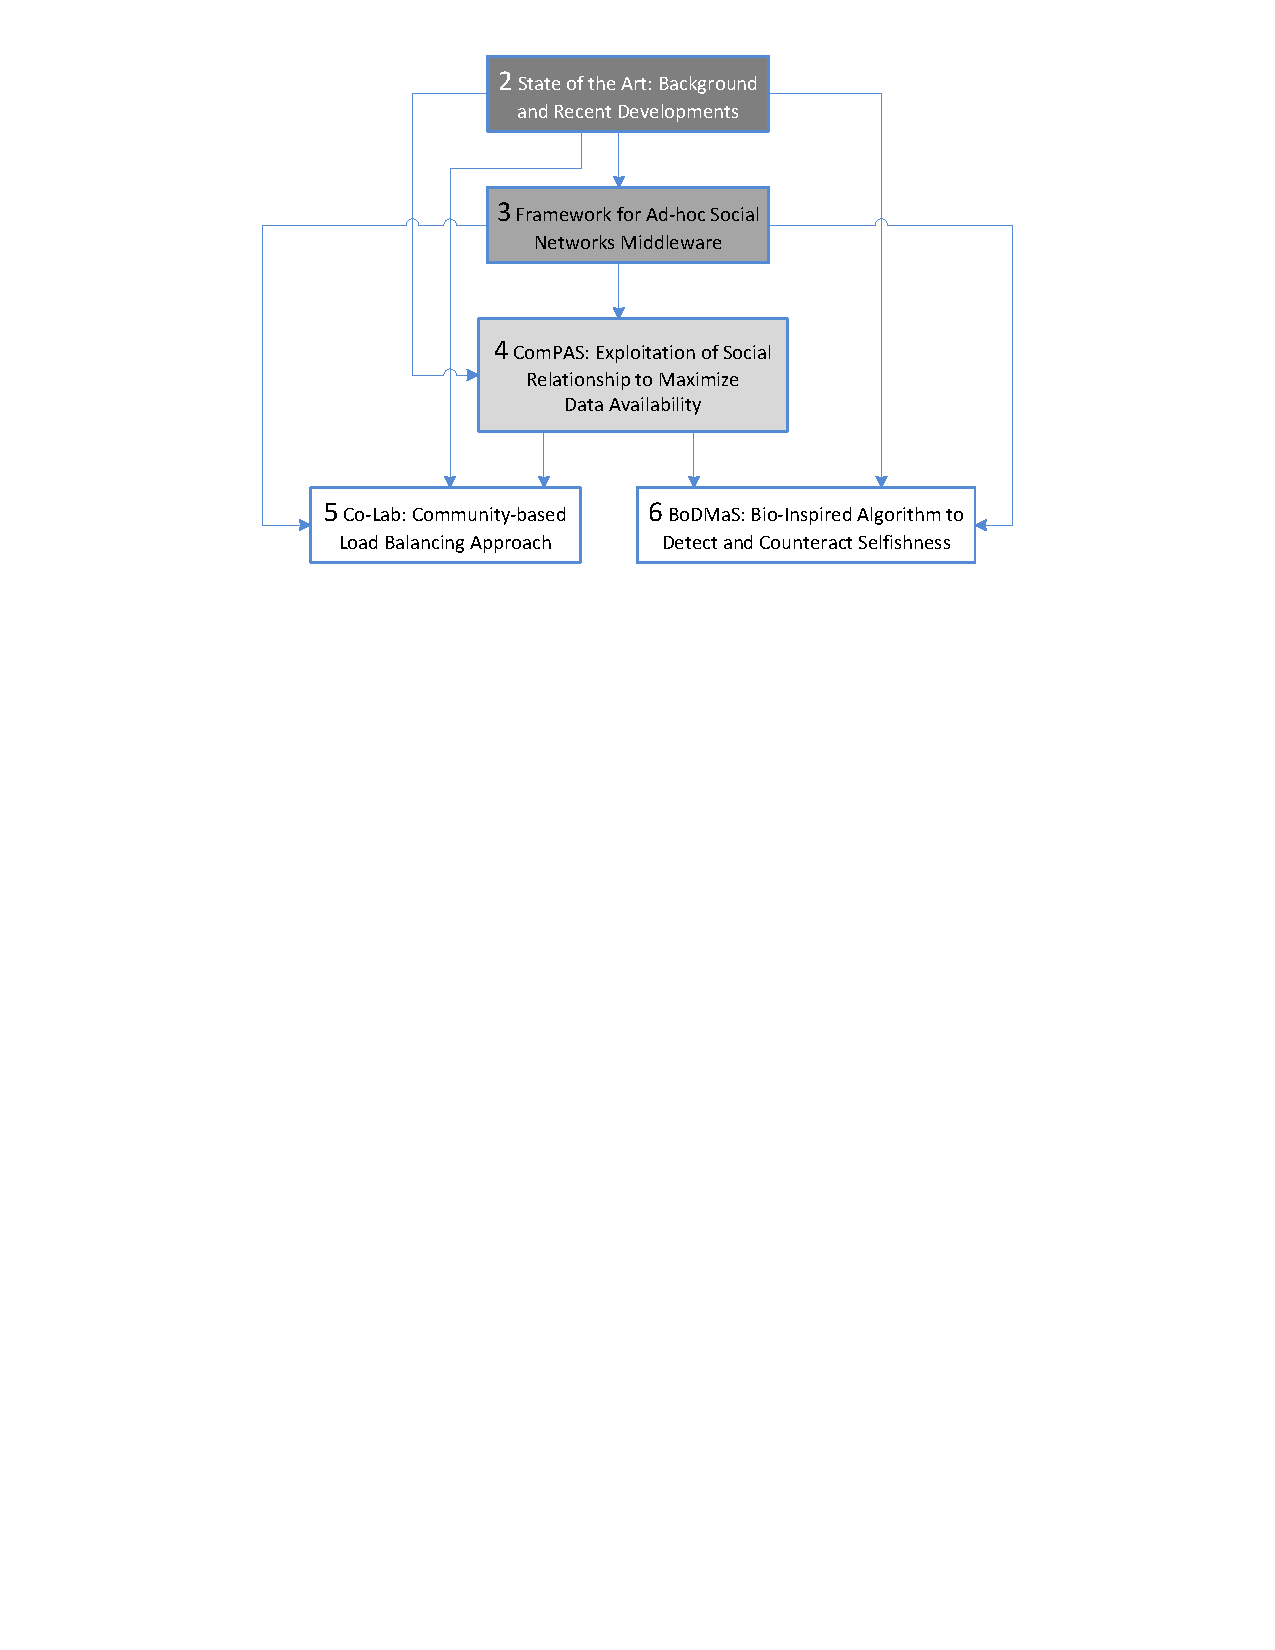
\includegraphics[width=0.75\textwidth]{Chap1-Fig3.pdf}
  \end{tabular}
  \caption{Dependency between dissertation Chapters. Arrows show dependencies and colors represent chapter levels.}
\end{center}
\end{figure}
